\documentclass[tikz]{standalone}

\usepackage{amsmath}
\usetikzlibrary{calc,angles,quotes}

\renewcommand{\vec}[1]{\boldsymbol{#1}}

\tikzset{>=latex}
\begin{document}
\begin{tikzpicture}
  \node[anchor=south west,inner sep=0] at (0,0) {
    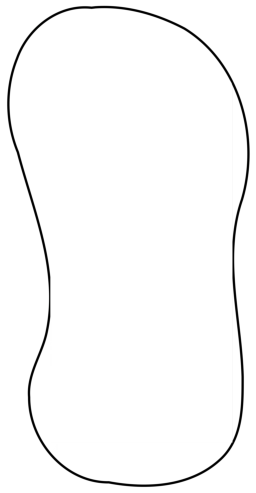
\includegraphics[width=\textwidth, angle=-20]{foot}};

   \begin{scope}[shift={(2.955,1.3)},rotate=0]
     \node[coordinate] (rf_center) at (6.5,10) {};
     \node[coordinate] (rf_y_final) at (9.5,10) {};
     \draw[->,ultra thick, blue] (rf_center)--(rf_y_final) node[right]{\huge $\vec{x}_{g}$};
     \draw[->,ultra thick, blue] (rf_center)--(6.5, 13) node[above]{\huge $\vec{y}_{g}$};
  \end{scope}

  
  \begin{scope}[shift={(-0.05,4.12)},rotate=-20]
    \node[coordinate] (foot_center) at (6.5,10) {};
    \node[coordinate] (zmp) at (10,16) {};
    \node[coordinate] (x_final) at (9.5,10) {};
    \node[coordinate] (y_final) at (6.5, 13) {};

    \draw[->,ultra thick, orange] (foot_center) -- (zmp);
    
    \draw[line width=0.5mm,red] (11,2.3) rectangle (2.4,19.5);
    \draw[black, fill=black] (foot_center) circle (4pt);
    \node[left=10, below=0, font=\sffamily] at (foot_center) {\huge $\vec{r}_k$};
    \draw[black, fill=black] (zmp) circle (4pt);

    \node[left=8, above=2, font=\sffamily] at (zmp) {\huge $\vec{p}_k$};
    \draw[->,ultra thick] (foot_center)--(x_final) node[right,font=\sffamily]{\huge $\vec{x}_{f}$};
    \draw[->,ultra thick] (foot_center)--(y_final) node[above, font=\sffamily]{\huge $\vec{y}_{f}$};
  \end{scope}

  \node[coordinate] (rf_y) at (9.5,15) {};  
  
  \pic [draw,ultra thick, <-, angle eccentricity=0, angle radius = 2cm] {angle = rf_y--rf_center--y_final};
  \node[left=1, below = 165] at (rf_y) {\huge $\alpha_k$};
  
\end{tikzpicture}
\end{document}
